\documentclass{article}
\usepackage[utf8]{inputenc}
\usepackage{titling}
\newcommand{\subtitle}[1]{%
  \posttitle{%
    \par\end{center}
    \begin{center}\large#1\end{center}
    \vskip0.5em}%
}
\usepackage{graphicx}
\usepackage{tikz}
\usepackage{setspace}
\usepackage{fancyhdr}
\usepackage{gensymb}
\usepackage{amsmath}
\usepackage{amsfonts}
\usepackage{amssymb}
\usepackage{parskip}
\usepackage{float}
\usepackage{gensymb}
\usepackage{amsthm}
\usepackage [english]{babel}
\usepackage [autostyle, english = american]{csquotes}
\MakeOuterQuote{"}
\usepackage{comment}

\pagestyle{fancy}
\fancyhf{}
\fancyhead[R]{\thepage}
\newcommand{\Z}{\mathbb{Z}}
\newcommand{\p}{\varphi}
\newcommand{\al}{\alpha}
\newcommand{\qrb}[2]{\big( \frac{#1}{#2}\big)}
\newcommand{\qrB}[2]{\Big( \frac{#1}{#2}\Big)}
\newcommand{\qrbg}[2]{\bigg( \frac{#1}{#2}\bigg)}
\newcommand{\qrn}[2]{\left( \frac{#1}{#2}\right)}

\begin{document}
\doublespacing
\title{Quadratic Residues in Olympiad Problems}
\subtitle{How can quadratic residues determine families of prime divisors?}
\date{}
\maketitle
\begin{center}
    Word count: 3886
    
    Subject: Mathematics
\end{center}
\newpage
\tableofcontents
\newpage
\section{Introduction}
\subsection{What is Number Theory?}
Number theory is the study of properties of positive integers. Its primary purpose is to "discover [and prove] interesting and unexpected relationships between different sorts of numbers,"\footnote{[1] Silverman.} for example the proof that there are infinitely many prime numbers and the proof that if a square number is divisible by two, it must be divisible by four.
\subsection{Why did I choose to investigate Quadratic Residues?}
When learning introductory Number Theory to strengthen my math contest skills, I was fascinated by how elegant modular arithmetic was. Eventually, I took a Number Theory course at a summer camp that introduced me to a variety of exciting and intricate concepts---order, p-adic valuation, multiplicative functions, Diophantine equations, and quadratic residues. However, I never understood quadratic residues very well, and thus believe that I missed out on a world of exploration.

Hence, I would like to use this essay to explore quadratic residues and deepen my own understanding. I will do this by solving olympiad-style questions and exploring my own extension.

This essay will first introduce modular arithmetic, then Euler's Totient Theorem, and then quadratic residues. The essay will then present my solution to a Taiwanese Olympiad problem in order to demonstrate applications and limitations of quadratic residues. Finally, this essay will focus on exploring a problem by Fermat, along with my own extension, on how quadratic residues can determine whether certain families of prime divisors exist.

The purpose of this essay is to demonstrate the usefulness of quadratic residues by exploring its use in Olympiad problems and by exploring relationships between sequences of numbers and families of prime factors.
\newpage
\section{Modular Arithmetic}
Modular arithmetic is foundational for number-theoretic exploration. To explain its properties, divisibility must first be defined.
\subsection{Divisibility}
Informally, $a$ divides $b$ if $\frac{b}{a}$ is both defined and an integer. However, in number theory, we do not often use rational numbers. Thus, the definition for divisibility is given below.

Let $a,b \in \Z$. Define $a$ divides $b$ if there exists $c\in \Z$ such that $ac = b$. This can be written as $a \mid b$. Notice that this definition allows for the inclusion of zero, despite division by zero being undefined. For example, we have $-2 \mid 10$ since $(-2) \cdot (-5) = 10$, $3 \mid 0$ since $3 \cdot 0 = 0$, and $0 \nmid 4$ because there is no integer $c$ that satisfies $0 \cdot c = 4$.

Notice that if $p$ is prime and $x,y \in \Z$, then if $p \mid xy$, then we must either have $p \mid x$ or $p \mid y$, since either $x$ or $y$ has to include the factor of $p$.
\subsection{Modular Arithmetic}
We must first define modular arithmetic because quadratic residues only make sense in such a context.
\subsubsection{Congruence}
Let $a,b,c \in \Z.$ Define $a \equiv b \pmod c$ --- read as $a$ is congruent to $b$ modulo $c$ --- if and only if $c \mid a-b$. Here, $c$ is defined as the modulus.

Note that this is equivalent to stating that if $a=cx+b$ for $x \in \Z$, then $a \equiv b \pmod c$ and vice versa. Also, note that if $d \in \Z$ is the remainder when $a$ is divided by $c$, then $a \equiv d \pmod c$. Here, $d$ is also known as a residue. For example, $29 \equiv -4 \equiv 2 \pmod 3$ since $29, -4,$ and $2$ each has a remainder and residue of $2$ when divided by 3. Alternatively, note that $3 \mid 29 - (-4) = 33$ and $3 \mid 2 - (-4) = 6$.

Modular arithmetic thus results in a cyclical nature, similar to the time of day. If there were a 12-hour analog clock currently showing 12 o'clock, the clock would show the same time if 5 hours passed, if 17 hours passed, or if $(5+12n)$ hours passed from the same starting time. Since the time on the clock repeats every twelve hours, the modulus is $12$. The statement above is akin to stating that $5 \equiv 5+12n \pmod {12}$.

The cyclical nature of modular arithmetic can be seen in the graph below.
\begin{figure}[H]
    \centering
    \begin{tikzpicture}
    \node[anchor=south west,inner sep=0] at (0,0) {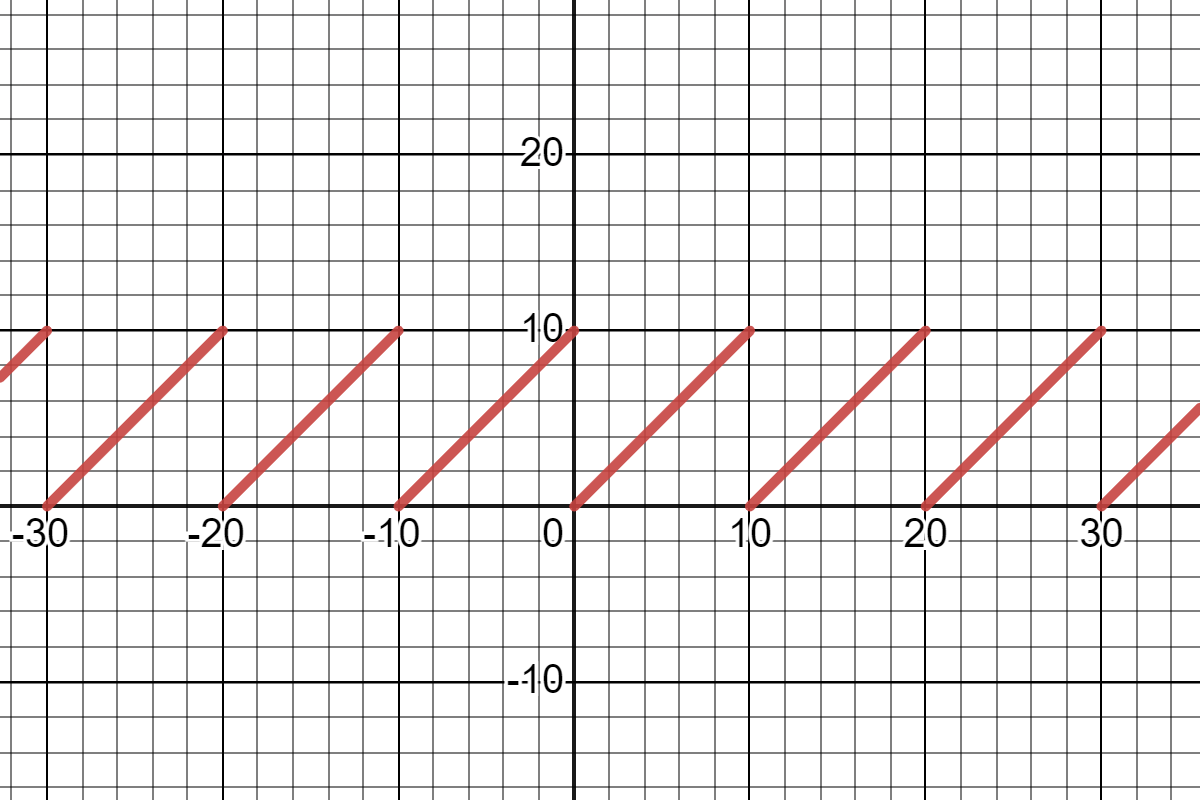
\includegraphics[width=\textwidth]{mod10.png}};
    \end{tikzpicture}
    \caption{A graph of $y=x-10\left\lfloor \frac{x}{10}\right\rfloor$ from Desmos. [3] "Graphing Calculator."}
\end{figure}
In this graph, all of the points with integral $x$-coordinates have the $y$ value of the residue of $x \pmod {10}$. While the graph has a $y$-value for each $x \in \mathbb{R}$, Number Theory focuses on integers. When restricting the domain to integers, we end up with the graph below.
\begin{figure}[H]
    \centering
    \begin{tikzpicture}
    \node[anchor=south west,inner sep=0] at (0,0) {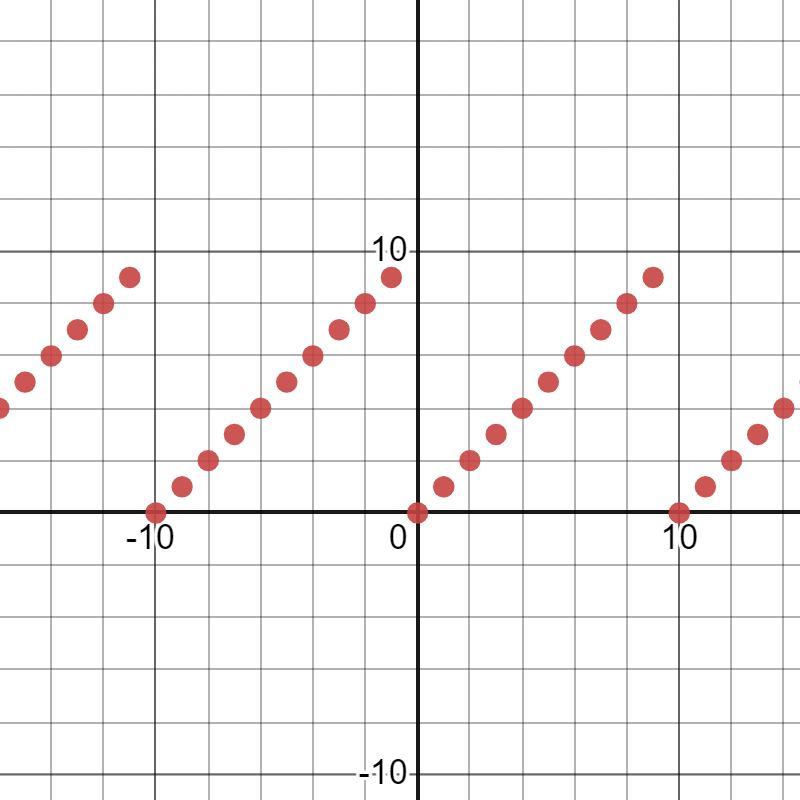
\includegraphics[width=\textwidth]{mod10 integers.png}};
    \end{tikzpicture}
    \caption{The same graph but restricted to integers. [3] "Graphing Calculator."}
\end{figure}
From the definition of modular arithmetic provided in this essay, only integral points are defined.
\subsubsection{Arithmetic Operations}
Let $a,b,m,n,k \in \Z$, where $k \ge 1$. Suppose that $a \equiv m \pmod k$ and $b \equiv n \pmod k$. Then, the following hold.\footnote{[2] Rusczyk.}
$$a+b \equiv m+n \pmod k.$$ For example, $12 + 23 \equiv 2 + 3 \equiv 5 \pmod {10}$.
$$a-b \equiv m-n \pmod k.$$ For example, $2-13 \equiv 2- 6 \equiv -4 \equiv 3 \pmod 7$.
$$ab \equiv mn \pmod k.$$ For example, $12 \cdot 17 \equiv 2 \cdot 7 \equiv 14 \equiv 4 \pmod{10}$, and  $16 \cdot 16 \equiv (-1) \cdot (-1) \equiv 1 \pmod {17}$.

For $x \in \Z,$ \[a^x \equiv m^x \pmod k.\] For example, $23^{2023} \equiv (-1)^{2023} \equiv (-1) \equiv 11 \pmod{12}$.

Notice that the addition, subtraction, and multiplication operators function as expected in modular arithmetic. However, notice that in exponentiation, only the base can be simplified by being taken modulo $k$.
\subsection{Fermat's Little Theorem}
Fermat's Little Theorem allows us to simplify the exponent in some certain cases. It is a special case of Euler's Totient Theorem in Appendix A. It states that for a prime $p$ and an integer $a$ such that $p \nmid a$, \[a^{p-1} \equiv 1 \pmod p.\]
For example, $10^{14} \equiv 10^2\cdot10^{13-1}\equiv 10^2\cdot 1 \equiv (-3)^2 \equiv 9\pmod{13}$.
\newpage
\begin{comment}
\section{Primitive Roots}
Define $g$ to be a primitive root$\pmod n$ if the set of integers $\{g, g^2, g^3, \cdots, g^{\p (n)}\}$ has the same residues as the set of integers $\{a_1, a_2, \cdots, a_{\p(n)}\}$, where $a_i$ for $1\le i \le \p(n)$ are the residues coprime to $n$.\footnote{See reference [8].}

For example, notice that 3 is a primitive root modulo 7 because the integers $3, 3^2, 3^3, \cdots, 3^6$ have residues $3, 2, 6, 4, 5, 1$, respectively, which is the set of all residues coprime to 7. However, 2 is not a primitive root modulo 7 because the integers $2, 2^2, 2^3, \cdots, 2^6$ have residues $2, 4, 1, 2, 4, 1$, respectively, which excludes residues such as 3 and 5.
\subsection{Properties}
Note that $g^{\p(n)} \equiv 1 \pmod n$ from Euler's Totient Theorem. However, notice that $\p(n)$ is the minimum exponent $x$ such that $g^{x} \equiv 1 \pmod n$. To prove this, suppose for the sake of contradiction that $y < \p(n)$ satisfies $g^y \equiv 1 \pmod n$. Then, consider the set of all residues of $g^k$ when varying $k$. There are at most $y$ unique values, as $g^k \equiv g^{k+cy} \pmod n$ for any integer $c$. Then, $\{g^1, g^2, \cdots, g^{y}\}$ are the only unique residues because $g^{y+1} = g^{y} \cdot g \equiv g$, resulting in a cycle. Since there are $y<\p(n)$ unique residues, $g$ cannot be a primitive root.

More intuitively, in order for a primitive root $g$ to cover all coprime residues, the sequence $g, g^2, g^3, \cdots$ modulo $n$ cannot repeat more than once every $\p(n)$ elements. Since Euler's Totient Theorem tells us that all residues $m$ when taken in the sequence $m, m^2, m^3, \cdots$ will repeat when the exponent is $\p(n)$, we know that the minimum exponent $x$ satisfying $g^x \equiv 1 \pmod n$ is $x=\p(n)$.

As a result, any residue $a_i$ coprime to $n$ can be written as $g^{j}$ for some $j \in \Z$.
\newpage
\end{comment}
\section{Quadratic Residues}
We will first define quadratic residues and then provide interesting properties. Intuitively, quadratic residues represent the perfect squares of a modulus.
\subsection{Definition}
Let $p$ be a prime. Consider all residues modulo $p$. Define a residue $a$ to be a quadratic residue modulo $p$ if there exists a solution to the equation $x^2 \equiv a \pmod p$. All residues that are not quadratic residues are considered quadratic non-residues. This can be expressed using the Legendre Symbol, which is defined as such.\footnote{[9] "Legendre Symbol."}
\[   \left( \frac{a}{p} \right) = \left\{
\begin{array}{ll}
      1 & \text{if }a \text{ is a quadratic residue modulo }p \text{ and } p \nmid a \\
      -1 & \text{if }a \text{ is a quadratic non-residue modulo }p\\
      0 & \text{if }p \mid a \\
\end{array} 
\right. \]
For example, consider the prime $p=13$. Each residue and it squared can be seen in the table below.
\begin{table}[H]
\centering
\begin{tabular}{|c|c|c|c|c|c|c|c|c|c|c|c|c|c|}
\hline
$x \bmod {13}$      & 0 & 1 & 2 & 3 & 4 & 5  & 6  & 7  & 8  & 9 & 10 & 11 & 12 \\ \hline
$x^2$ & 0 & 1 & 4 & 9 & 16 & 25 & 36 & 49 & 64 & 81 & 100  & 121  & 144  \\ \hline
$x^2\bmod {13}$ & 0 & 1 & 4 & 9 & 3 & 12 & 10 & 10 & 12 & 3 & 9  & 4  & 1  \\ \hline
\end{tabular}
\end{table}
Then, the set of quadratic residues is $\{0, 1, 3, 4, 9, 10, 12\}$ --- so for example $\qrn{12}{13}=1$ --- and the set of quadratic non-residues is $\{2, 5, 6, 7, 8, 11\}$ --- so for example $\qrn{2}{13}=-1$.

Notice that if $\qrn{a}{p} = 1$, then $\qrn{a+np}{p} = 1$, and $\qrn{a}{p} = -1 \iff \qrn{a+np}{p} = -1$ for $n \in \Z$. This is because if $x^2 \equiv a \pmod p$, then $x^2 \equiv a + np \equiv a \pmod p$. For example, $\qrn{15}{13} =\qrn{2}{13}=-1$.

Another interesting property is that there are $\frac{p-1}{2}$ non-zero quadratic residues and $\frac{p-1}{2}$ quadratic non-residues.\footnote{[10] “Number of Quadratic Residues of Prime.”} To see why, note that
\[q^2 \equiv r^2 \pmod p \iff q^2 - r^2 \equiv 0 \iff (q-r)(q+r) \equiv 0 \iff q \equiv \pm r.\]
Then, each non-zero quadratic residue has exactly two unique non-zero residues that square to it. Since there are $p-1$ non-zero residues, there are $\frac{p-1}{2}$ unique quadratic residues and thus $p-1 - \frac{p-1}{2} = \frac{p-1}{2}$ quadratic non-residues.

Indeed, in the example with $p=13$, we find $\frac{13-1}{2}=6$ non-zero quadratic residues and $\frac{13-1}{2}=6$ quadratic non-residues.
\subsection{Euler's Criterion}
Euler's Criterion\footnote{[11] “Euler's Criterion.”} provides a way to calculate the Legendre symbol with modular exponentiation. It states that for a prime $p$,
\[\left(\frac{a}{p}\right) \equiv a^{\frac{p-1}{2}} \pmod p.\]
We will establish intuition as to why this is true.

When $p=2$, this is verifiable.

Assume that $p$ is odd. Then, from Fermat's Little Theorem,
\begin{align*}a^{p-1} \equiv 1 \pmod p &\implies (a^{p-1}-1) \equiv 0 \pmod p \\ &\implies (a^{\frac{p-1}{2}}-1)(a^{\frac{p-1}{2}}+1) \equiv 0 \pmod p.\end{align*}
Since the product is congruent to 0, one of the factors must be 0.
Suppose $\qrn{a}{p}=1$. Then, there exists $x$ such that $x^2 \equiv a \pmod p$. Then, $a^{\frac{p-1}{2}} \equiv x^{p-1} \equiv 1$ by Fermat's Little Theorem.

Now suppose $\qrn{a}{p}=-1$. In this case, the $x$ above does not exist. Then, intuitively, $a^{\frac{p-1}{2}} -1 \not\equiv 0 \pmod p$ but as found above, $(a^{\frac{p-1}{2}}-1)(a^{\frac{p-1}{2}}+1) \equiv 0 \pmod p \implies a^{\frac{p-1}{2}} +1 \equiv 0 \implies a^{\frac{p-1}{2}} \equiv -1 \pmod p$, meaning that if $a$ is not a quadratic residue, we should have $a^{\frac{p-1}{2}} \equiv -1 \pmod p$.

This does not formally prove Euler's Criterion because it is not established that for quadratic non-residues, $a^{\frac{p-1}{2}} -1 \not \equiv 0$. However, sufficient intuition has been established.

\begin{comment}
Suppose that $a^\frac{p-1}{2} \equiv 1 \pmod p$. Then, suppose $g$ is a primitive root modulo $p$, where $g^j \equiv a \pmod p$. Then, $g^{j \cdot \frac{p-1}{2}} \equiv 1 \pmod p$. However, we know that since $g$ is a primitive root, $\p(p) = p-1$ is the minimum integer $x$ such that $g^x \equiv 1$, which implies that $p-1 \mid j \cdot \frac{p-1}{2}$. Then, $j$ must be an even integer. If we let $j=2k$, then we have $a^{\frac{p-1}{2}} \equiv (g^{j})^{\frac{p-1}{2}} \equiv (g^{\frac{p-1}{2}})^j \equiv (g^{k\cdot \frac{p-1}{2}})^2 \equiv a \pmod p$, which must mean that $a$ is a quadratic residue. Thus, we have proven that $a$ is a quadratic residue if and only if $a^{\frac{p-1}{2}} \equiv 1 \pmod p$. Then, if $a$ is a quadratic non-residue, then $a^{\frac{p-1}{2}}$ must be congruent to $-1 \pmod p$.
\end{comment}

\subsection{Multiplicativity}
A consequence of Euler's Criterion is that for $b,c\in\Z$ and $p$ is a prime, then \[\qrbg{b}{p}\qrbg{c}{p} = \qrbg{bc}{p}.\]
This can be proven as follows.\footnote{[13] Andreescu and Dospinescu 402.} \[\qrn{bc}{p}=(bc)^{\frac{p-1}{2}} \equiv b^{\frac{p-1}{2}}\cdot c^{\frac{p-1}{2}} \pmod {p} = \qrbg{b}{p}\qrbg{c}{p}.\]

For example, when $p=13$, the set of quadratic residues is $\{0, 1, 3, 4, 9, 10, 12\}$ and the set of quadratic non-residues is $\{2, 5, 6, 7, 8, 11\}$. Notice that $\qrn{3}{13}\qrn{5}{13} = \qrn{15}{13} = \qrn{2}{13} = (1)(-1) = -1$, which agrees with our sets.
\subsection{Quadratic Reciprocity Law}
The Quadratic Reciprocity Law\footnote{[12] "Law of Quadratic Reciprocity."} states that for two distinct odd primes $p, q,$
\[\qrbg{p}{q} \qrbg{q}{p} = (-1)^{\frac{(p-1)(q-1)}{4}}.\]
However, in my exploration, I found a more useful representation that will be used in our proofs. Since these two primes are distinct, $\qrn{q}{p} = \pm 1$. Then, $\big(\frac{q}{p}\big)^2=1$. Multiplying both sides by $\big(\frac{q}{p}\big)$ yields
\[\tag{Quadratic Reciprocity}\qrbg{p}{q} = \qrbg{q}{p}(-1)^{\frac{(p-1)(q-1)}{4}}.\]
For example, suppose we wish to calculate $\qrn{37}{73}$. Quadratic reciprocity yields
\[\qrn{37}{73} = \qrn{73}{37}(-1)^{\frac{(73-1)(37-1)}{4}}=\qrn{73}{37}=\qrn{36}{37}=\qrn{6}{37}\qrn{6}{37}=\qrn{6}{37}^2 = 1.\]
Notice that any Legendre symbol can be simplified by using Quadratic Reciprocity, then reducing the top  modulo the bottom, factoring, and then repeating until both arguments are small enough to be calculated manually.
\newpage
\section{The Taiwanese Olympiad Problem}
This problem is from the 1997 Taiwanese Olympiad\footnote{[13] Andreescu and Dospinescu 419.}:
\begin{center}
Let $k=2^{2^n}+1$ for some positive integer $n$. Prove that \\ $k$ is a prime if and only if $k$ is a factor of $3^{\frac{k-1}{2}}+1$.
\end{center}
This problem asks to prove an "if and only if" statement. To do so, I considered the "if" and the "only if" parts separately. I started with the "only if" part since it seemed easier.
\subsection{Proving the "only if" direction}
The "only if" statement wishes for us to assume that $k=2^{2^n}+1$ is a prime, and then prove that $k \mid 3^{\frac{k-1}{2}} + 1$.

I noticed that the statement we wish to prove is equivalent to $3^{2^{2^n-1}} \equiv -1 \pmod{2^{2^n}+1}$.
This looks similar to Euler's Criterion. In fact, the equivalent statement in terms of $k$ is $3^{\frac{k-1}{2}} \equiv -1 \pmod k$.

Since $k$ is prime, Euler's Criterion can directly be applied, resulting in $\qrn{3}{k} \equiv -1$. Quadratic reciprocity states
\[\qrbg{p}{q} = \qrbg{q}{p}(-1)^{\frac{(p-1)(q-1)}{4}}.\]
With $p=3, q=k$, this yields
\[\qrbg{3}{k}=\qrbg{k}{3} (-1)^{\frac{(3-1)(k-1)}{4}}=\qrbg{k}{3}(-1)^{2^{2^n-1}}=\qrbg{k}{3}=-1.\]
Note that $(-1)^{2^{2^n-1}}=1$ for all $n \in \Z^+$. Then, $\qrn{k}{3} = -1 \iff k \equiv 2 \pmod 3$.

Since all of these steps are reversible, it suffices to prove that $k \equiv 2 \pmod 3$ to solve the "only if" direction. We have \[k = 2^{2^n}+1 \equiv (-1)^{2^n}+1 = ((-1)^2)^{2^{n-1}}+1 = 1^{2^{n-1}}+1 \equiv 1+1 \equiv 2 \pmod 3.\]
Note that the first equivalence is true because $2^a \equiv (-1)^a \pmod 3$ for $a \in \Z$.

Thus, the "only if" direction is complete. 

This part of the problem demonstrates how concepts in quadratic residues can be used in direct applications to number-theoretic olympiad problems. 

\subsection{Proving the "if" direction}
We will first introduce a useful lemma.

\subsubsection{Minimum exponent lemma}
\paragraph{Lemma} Define $x \in \Z^+$ to be the minimum integer satisfying $a^x \equiv 1 \pmod b$, where $a, b \in \Z$ such that $\gcd(a, b) = 1$. Then, all integers $y$ satisfying $a^y \equiv 1 \pmod b$ must be divisible by $x$.

The proof is in Appendix C, but here is a diagram to give intuition for the lemma.
\paragraph{Intuition}
\begin{figure}[H]
    \centering
    \begin{tikzpicture}
    \node[anchor=south west,inner sep=0] at (0,0) {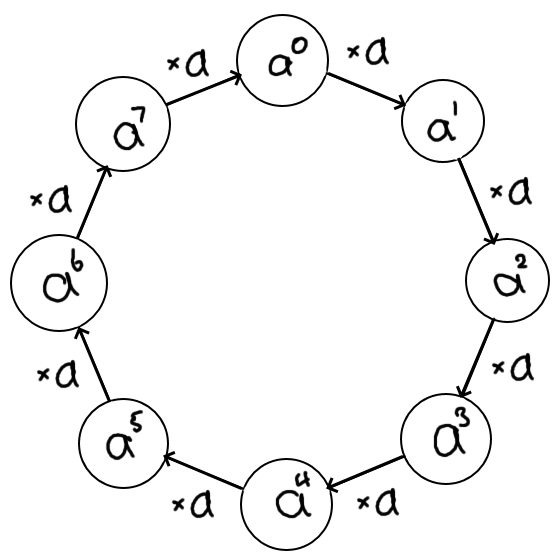
\includegraphics[width=8cm]{diagram1.png}};
    \end{tikzpicture}
    \caption{An example where $x=8$. $a^1, a^2, \cdots, a^7 \neq 1$.}
\end{figure}

Imagine beginning at $a^0$ and going forwards in the cycle $y$ times. The expression $a^y$ is only congruent to $1$ if $a^y$ travels a complete number of cycles, implying that $x \mid y$, where $x$ is the minimum cycle length.

\subsubsection{The proof}
The "if" statement wishes for us to assume that $k = 2^{2^n}+1 \mid 3^{\frac{k-1}{2}}+1$, and then prove that $k$ is prime.

I originally tried proof by contradiction. However, this did not lead anywhere useful. I then considered a prime factor $p$ of $k$, with the goal of proving that $p$ must necessarily be $k$, which would prove that $k$ is prime.

I noticed that we had $k \mid 3^{\frac{k-1}{2}}+1 \iff 3^{\frac{k-1}{2}} \equiv -1 \pmod k$. Since $p \mid k$, we must also have $p \mid 3^{\frac{k-1}{2}}+1 \iff 3^{\frac{k-1}{2}} \equiv -1 \pmod p$. I noticed that $3^{\frac{k-1}{2}} 
\equiv -1 \pmod p$ looks similar to Euler's Criterion, but it cannot be used here, since we do not know that the $k$ in the exponent is equal to the modulus $p$.

Instead, I used $k = 2^{2^{n}}+1$ and squared both sides of the congruence below to arrive at
\[3^{\frac{k-1}{2}} 
\equiv 3^{2^{(2^n-1)}} \equiv -1 \pmod p \implies 3^{2^{2^n}} \equiv 1 \pmod p.\]

Let $x$ be the minimum exponent with $3^x \equiv 1 \pmod p$. Because $3^{2^{2^{n}}} \equiv 1 \pmod p$ from above, $x \mid 2^{2^{n}}$ by the lemma. However, since $3^{2^{(2^{n}-1)}} \equiv -1 \pmod p$, we must have $x \nmid 2^{(2^n-1)}$. The only value of $x$ satisfying these two conditions is $x = 2^{2^n}$.

Additionally, $3^{p-1} \equiv 1 \pmod p$ by Fermat's Little Theorem, and $x \mid p-1$ by the lemma. Therefore, $x =  2^{2^{n}} \le p-1 \implies p \ge 2^{2^n}+1$. 

However, from the definition of $p$, we have $p \mid k \implies p \mid 2^{2^n}+1 \implies p \le 2^{2^n}+1$. The only value of $p$ satisfying both inequalities is $p=k$, implying that $k$ is prime.

Thus, both directions of the problem have been proven. \qedsymbol

Even though the problem seems to be closely related to quadratic residues, this part demonstrates that quadratic residues were not able to be applied just by changing the direction of proof required. Thus, quadratic residues have their limitations in number theory questions.
\newpage
\section{Fermat's Problem}
We will explore some general complex divisibility properties through a problem by Fermat.
\begin{center}
     Prove that the numbers $3^n + 1$ have no divisor of the form $12k + 11$.\footnote{[13] Andreescu and Dospinescu 422.}
\end{center}
\subsection{Proof of Simpler Version}
\label{proofsimpler}
I wish to first solve a simpler version to develop insights. To do so, I assume that the divisor $12k + 11$ is prime. Thus, I will prove that the numbers $3^n + 1$ have no prime divisor of the form $12k + 11$. This will be accomplished by assuming that $3^n + 1$ has a prime divisor of the form $12k+11$ to arrive at a contradiction.

First, note that if $3^n+1$ has a prime divisor of the form $p=12k+11$, then $p \mid 3^n + 1 \Rightarrow 3^n+1 \equiv 0 \pmod p \Rightarrow 3^n \equiv -1 \pmod p$.

We wish to use quadratic residues to arrive at a contradiction.
\begin{comment}
My first attempt at this was squaring both sides, resulting in $3^{2n} \equiv 1 \pmod p$. However, since $1$ is a perfect square, it is also a quadratic residue. I first considered applying the concept of the minimum value of $x$ such that $3^x \equiv 1 \pmod p$; however, this did not lead anywhere.
\end{comment}

I noticed that if $n \equiv 0 \pmod 2$, then quadratic residues could be applied, because then $n=2k, \hspace{2pt} k \in \Z$, so $3^n \equiv 3^{2k} \equiv (3^{k})^2 \equiv -1 \pmod p$, implying that $-1$ is a quadratic residue. However, using Euler's Criterion, \[\left(\frac{-1}{p}\right)=(-1)^{\frac{p-1}{2}}=(-1)^{\frac{(12k+11)-1}{2}}=(-1)^{6k+5}=(-1),\] implying that $-1$ is a quadratic non-residue modulo $p$. Thus, we have arrived at a contradiction if $n$ is even.

Hoping to use a similar argument to arrive at a contradiction, I assumed that $n \equiv 1 \pmod 2$ to complete the casework.

We still have $\qrn{-1}{p}=(-1)$ from above. Then, $n=2k-1, \hspace{2pt} k\in \Z$. This gives $3^{n} \equiv 3^{2k-1} \equiv -1 \pmod p$. Wanting to use quadratic residues, I multiplied both sides by $3$ to get $3^{2k} \equiv -3 \pmod p$, implying that $-3$ is a quadratic residue modulo $p$. Using multiplicity of the Legendre symbol and Euler's Criterion gives $\left(\frac{-3}{p}\right)= \left(\frac{3}{p}\right)\left(\frac{-1}{p}\right)=-\qrn{3}{p}$. Using the Quadratic Reciprocity Law with $p=12k+11$ gives \[\qrn{-3}{p}=-\Big(\frac{3}{p}\Big)=-\qrn{p}{3}(-1)^{\frac{(3-1)(p-1)}{4}}=-\qrn{p}{3}(-1)^{6k+5}=\qrn{p}{3}.\] We also have $\left(\frac{p}{3}\right) = \left(\frac{12k+11}{3}\right) = \left(\frac{2}{3}\right)=-1$, since $2$ is a quadratic non-residue modulo $3$. Thus, we have $\qrn{-3}{p}= \qrn{p}{3}=-1$, meaning that $-3$ is a quadratic non-residue modulo $p$, which is a contradiction if $n$ is odd.

A contradiction has been established in both cases; thus, the framework for the proof is complete.

\subsection{Proof}
To solve the full problem, we assume that $x\equiv 11 \pmod {12}$ is a factor of $3^n+1$ for the sake of contradiction. Writing $x$ in terms of its prime factors gives \[x = \prod_{i=1}^{y} p_i^{\al_i}\equiv 11 \pmod{12}.\]
An important observation is that since $11$ and $12$ are coprime, no $p_i$ can be 2 or 3. This is because if some $p_k=2$, then $2 \mid x$. However, $x \equiv 11 \pmod{12} \implies x \equiv 1 \pmod 2$, which gives us a contradiction. The same argument applies to 3.

Thus, each of the prime factors $p_i$ can only be congruent to $1, 5, 7,$ or $11 \pmod {12}$, because all other residues are divisible by either 2 or 3.

Consider $p_i$, a specific prime divisor of $x$. Suppose $x=p_i k, \hspace{2pt} k\in \Z$. Then, \begin{align*}3^n \equiv -1 \pmod x & \implies x \mid 3^n+1 \\ \implies p_i k \mid 3^n+1  \implies p_i \mid 3^n +1 & \implies 3^n \equiv -1 \pmod {p_i}.\end{align*} Note that this argument applies to all prime factors of $x$. This means that we can essentially reduce the modulus $x$ to one of its divisors $p_i$.

Now, we consider two cases. We first find all possible factors $x$ modulo 12 of $3^n+1$ when $n \equiv 0 \pmod 2$, and then when $n \equiv 1 \pmod 2$, and show that in both cases, $x\equiv 11$ is impossible.

When $n$ is even, we have $n=2k \implies 3^{2k}\equiv -1 \pmod {p_i}$, meaning that $-1$ is a quadratic residue modulo $p_i$. By Euler's Criterion, \[\left(\frac{-1}{p_i}\right)=(-1)^{\frac{p_i-1}{2}}=1 \implies p_i \equiv 1 \pmod 4.\]

Of the possible residues $1, 5, 7, 11 \pmod {12}$, only $1, 5$ are congruent to $1 \pmod 4$. Then, the prime factors that multiply to $x$ must only have residues $1, 5 \pmod {12}$.

Then, $x \equiv 1^{\beta_1} \cdot 5^{\beta_2} \equiv 5^{\beta_2} \pmod {12}, \hspace{2pt} \beta_1, \beta_2 \in \Z$.

However, when varying $\beta_2$, $x \equiv 5^{\beta_2}$ cycles between 5 and 1. Thus, the set of all possible residues for $x \pmod {12}$ are $\{1,5\}$ when $n$ is even.

The second case is slightly more involved. Here, we have $n = 2k-1, k \in \Z$. Then, $3^{2k} \equiv -3 \pmod x$ by multiplying both sides by $3$, so $\qrn{-3}{p_i} = 1$.

Using multiplicity, we have \[\left(\frac{-3}{p_i}\right)=\left(\frac{3}{p_i}\right) \left(\frac{-1}{p_i}\right) = 1.\]
Since the product is non-zero, we know that $p_i \nmid 3 \implies p_i \neq 3$.
Using the Quadratic Reciprocity Law gives \[\qrbg{3}{p_i} =\qrbg{p_i}{3}(-1)^{\frac{(3-1)(p_i-1)}{4}}=\qrbg{p_i}{3}(-1)^{\frac{p_i-1}{2}},\] and Euler's Criterion gives
\[\left(\frac{-1}{p_i}\right)=(-1)^{\frac{p_i-1}{2}}.\]
Then, \[\left(\frac{-3}{p_i}\right)=\left(\frac{3}{p_i}\right) \left(\frac{-1}{p_i}\right) = \left(\qrbg{p_i}{3}(-1)^{\frac{p_i-1}{2}}\right)\left((-1)^{\frac{p_i-1}{2}}\right) = \qrbg{p_i}{3} (-1)^{p_i-1}.\]
Since $p_i$ is an odd prime, we have
\[\qrn{-3}{p_i} = \qrbg{p_i}{3} (-1)^{p_i-1} = \qrbg{p_i}{3}= 1.\]
This only occurs when $p_i \equiv 1 \pmod 3$, giving only $p \equiv 1, 7 \pmod{12}$ as our options.

We let $x \equiv 1^{\beta_1} \cdot 7^{\beta_2} \equiv 7^{\beta_2} \pmod{12}, \beta_1, \beta_2 \in \Z$. Similar to the first case, when varying $\beta_2$, $x$ cycles between 7 and 1. Thus, the set of all possible residues for $x \pmod {12}$ are $\{1,7\}$ when $n$ is odd.

Thus, the set of all possible residues of $x \pmod{12}$ is $\{1, 5, 7\}$, contradicting our assumption of the existence of $x \equiv 11 \pmod {12}$ and completing our proof.

In this problem, we began by looking at a simpler version for only prime numbers that provided a framework for the more general problem even though interestingly, the original problem does not mention primes. Quadratic residues were used by considering in separate cases the parity of the exponent to eliminate possible options and ultimately arrive at a contradiction.

\section{Extension}
\label{extension}
I made my own extension of the simpler version of the problem.
\begin{center}
    Find all triplets $(a,b,c)$, where $a, b, c \in \Z^+$ such that the \\ numbers $a^n+1$ have no prime divisor of the form $bk+c$.
\end{center}
%todo: have mini introductions and conclusions to keep the purpose clear
In my exploration, I try to find solutions by constructing a proof by contradiction, and noticing the necessary conditions on $(a,b,c)$ for the contradiction to work. I first follow my steps in the original question to derive the most general conditions for this new problem. Then, I try to find specific families of triplets by considering the case when $\gcd(b,c) > 1$, and when $\gcd(b,c) = 1$. In the second case, I experiment with gradually more general cases for $a$---first an odd prime, then a power of an odd prime, then a product of two powers of odd primes, and then finally any odd number.

\subsection{Deriving General Conditions}
Our goal is to find general conditions which satisfy the problem to pinpoint specific families of triplets $(a,b,c)$.

Hoping to use a similar line of reasoning as with the original problem, we let $p=bk+c$ and assume for the sake of contradiction that $a^n+1 \equiv 0 \pmod p$. Then, if the triplet $(a,b,c)$ is constructed in a way so that quadratic residues can be used to arrive at a contradiction, then the triplet satisfies the question.

We perform casework on the parity of $n$. However, for the proof to work, there must be a contradiction in both cases.

\paragraph{Case 1}: If $n=2k, \hspace{2pt} k \in \Z$, then $a^{2k} \equiv -1 \pmod p$, implying that $\qrn{-1}{p} = 1$. To mimic the contradiction in the original problem, we assume that \[\qrn{-1}{p} = -1 \implies (-1)^{\frac{p-1}{2}} = -1 \implies p = bk+c \equiv 3 \pmod 4.\] To guarantee this condition for all $k$, we must have $4 \mid b$ and $c \equiv 3 \pmod 4$.

\paragraph{Case 2}: If $n = 2k-1, \hspace{2pt} k \in \Z$, then \[a^{n} = a^{2k-1} \equiv -1 \pmod p \implies a^{2k} \equiv -a \pmod p \implies \qrn{-a}{p} = 1.\] To create a contradiction, we assume that $\qrn{-a}{p}=\qrn{-1}{p}\qrn{a}{p}=-1$. Since $\qrn{-1}{p}$ is assumed to be $-1$ from case 1, we must have $\qrn{-a}{p}=-1 \cdot \qrn{a}{p}=-1 \iff \qrn{a}{p} = 1$ for all $p$ in order to have a contradiction.

\textbf{To summarize, we need 3 key conditions to guarantee that the proof by contradiction works}: 
\begin{enumerate}
    \item $4 \mid b$
    \item $c \equiv 3 \pmod 4$
    \item $\qrn{a}{p}=1$ for all primes $p=bk+c$
\end{enumerate}

Indeed, in the original simplified problem, we have $a=3, b=12, c=11$, which satisfy these three conditions. The third condition is proven in section \ref{proofsimpler}.

Thus, the arguments in section \ref{proofsimpler} easily extend to this general extension to provide necessary conditions. However, from here new challenges appear.
\subsection{Finding Families of Triplets}
The remainder of this extension focuses on finding more specific conditions on $a,b,c$ that guarantees the conditions above. We will consider $\gcd(b,c)>1$ and $\gcd(b,c)=1$ separately as mentioned at the beginning of section \ref{extension}. Because this is very exploratory, many of these sections divide into further subcases.

\subsubsection{Case: $\gcd(b,c)>1$}
The problem statement matters only when $bk+c$ is prime. If $\gcd(b,c)>1$, I noticed that $bk+c$ can only be prime if $k=0$ and $c$ is prime. Otherwise, the expression $bk+c$ has at least 3 distinct factors: $1, \gcd(b,c),$ and $bk+c$, so it cannot be prime.

Thus, we can satisfy the key conditions with the following:
\begin{enumerate}
    \item $4\mid b$
    \item $c \equiv 3\pmod 4$
    \item $\qrn{a}{c}=1$, because $\qrn{a}{p}=\qrn{a}{bk+c}=\qrn{a}{b(0)+c}=\qrn{a}{c}$
    \item $c$ is prime
    \item $c\mid b$, because $c$ is prime and $\gcd(b,c)>1$
\end{enumerate}
These produce a family of solutions (family 1 in section \ref{foundfamilies}). This is the only family found by assuming that $b,c$ are not coprime, and so the rest of this extension will assume that $\gcd(b,c) = 1$.

\subsubsection{Case: $\gcd(b,c)=1$, $a$ is an odd prime}
Note that since $4\mid b, c \equiv 3 \pmod 4$ by the key conditions and $p = bk + c$, $p$ can be written as $p=4x+3, x \in \Z$. Then, Quadratic Reciprocity yields \[\qrn{a}{p} = \qrbg{p}{a}(-1)^{\frac{(a-1)(p-1)}{4}} = \qrbg{p}{a} (-1)^{\frac{(a-1)(4x+2)}{4}} = \qrbg{p}{a} (-1)^{\frac{(a-1)(2x+1)}{2}} = 1.\]
Notice that \[(-1)^{\frac{(a-1)(2x+1)}{2}}=((-1)^{2x+1})^\frac{a-1}{2} = (-1)^{\frac{a-1}{2}}.\]
Then,
\begin{equation}
\label{maineq}
\qrn{a}{p} = \qrbg{p}{a} (-1)^{\frac{(a-1)}{2}} = 1.
\end{equation}
To ensure that equation \ref{maineq} is always true, we will perform further casework on $a$.

\paragraph{Subcase 1 -- $a \equiv 1 \pmod 4$, $\gcd(a,b)=1$:} Here, $a\equiv 1\pmod 4 \implies (a-1)/2$ is even and $(-1)^{\frac{(a-1)}{2}}=1$. From equation 1, \[\qrbg{p}{a} (-1)^{\frac{(a-1)}{2}} = \qrbg{p}{a}=1.\] In other words, in order for the key conditions to be satisfied, $\qrn{p}{a}$ must be $1$ for all $p=bk+c$. 

I noticed that if $b$ and $a$ shared no common factors, then the sequence of integers $bk+c$ would be surjective modulo $a$. In other words, for every residue $x$ modulo $a$, there exists a value of $k$ such that $bk+c \equiv x \pmod a$. This turns out to be true even if only prime $bk+c$ are considered.

\paragraph{Surjectivity Lemma:} The primes of the form $p=bk+c$, when taken modulo an odd prime $a$ where $a \nmid b$, covers all non-zero residues modulo $a$ infinitely many times.
\begin{comment}
\paragraph{Proof of Key Lemma}: I wish to apply Dirichlet's Theorem on Arithmetic Progressions\footnote{See reference [14].}, which states that for $a, d \in \Z$ such that $\gcd(a,d) = 1$, there are infinitely many primes of the form $a \pmod d$, or in other words, there are infinitely many primes in the arithmetic sequence $a+kd, k \in \Z$. To do so, I must first find the arithmetic sequence for each of the residues $x$ in the above paragraph.

We have $k \equiv (x-c)b^{-1} \pmod a$, meaning that $k = (x-c)b^{-1} + ay$ for $y \in \Z$. Plugging this back into $bk+c$ yields \[bk+c = b((x-c)b^{-1}+ay)+c = bb^{-1}(x-c) + aby+c \equiv x \pmod a,\] where $y$ varies and the other variables are constant. Then, in this arithmetic progression, we have the common difference as $ab$, and the first term as \\ $bb^{-1}(x-c)+c$. This arithmetic sequence has infinitely many primes if \\ $\gcd(ab, bb^{-1}(x-c)+c) = 1$. Since $a, b$ are coprime, the condition above is equivalent to the two conditions $\gcd(a, bb^{-1}(x-c)+c)=1$ and \\$\gcd(b, bb^{-1}(x-c)+c)=1$. Since $bb^{-1}(x-c)+c \equiv (x-c)+c \equiv x \pmod a$, this condition holds true if $x \neq 0 \pmod a$. Due to the Euclidean Algorithm, $\gcd(b, bb^{-1}(x-c)+c) = \gcd(b, c)=1$. Thus, primes of the form $bk+c$ will cover all non-zero residues modulo $a$, proving the lemma. \qedsymbol
\end{comment}

The proof of this lemma is lengthy and involves Dirichlet's Theorem\footnote{[14] Weisstein.}, but can be found in Appendix D.

The surjectivity lemma shows that if $a$ and $b$ are coprime, $\qrn{p}{a}$ cannot always be $1$. This is because there are $\frac{p-1}{2}$ non-zero quadratic residues and $\frac{p-1}{2}$ quadratic non-residues, and so primes of the form $bk+c$ must cover both quadratic residues and non-residues, which would result in the existence of a $\qrn{p}{a}=\pm 1 \implies \qrn{a}{p}=-1$, so the proof by contradiction does not necessarily work.

We have just shown that in this subcase, the proof by contradiction does not work. Thus, for $a\equiv 1\pmod 4$, we must have $\gcd(a,b)>1$ to find more families of triplets $(a,b,c)$ that satisfy the key conditions.

\paragraph{Subcase 2 -- $a \equiv 3 \pmod 4, \gcd(a,b)=1$:} By equation $(1)$, we must have $\qrn{p}{a}=-1$ for all values of $p$. The argument above using the surjectivity lemma still applies, showing that if $\gcd(a,b)=1$, then the proof by contradiction fails.

\paragraph{Subcase 3 -- $\gcd(a,b) > 1$:}
Since $a$ is prime, we must have $a \mid b \implies p = bk+c \equiv c \pmod a$. Then, equation 1 yields
\[\qrbg{p}{a} (-1)^{\frac{a-1}{2}} = \qrbg{bk+c}{a} (-1)^{\frac{a-1}{2}} = \qrbg{c}{a} (-1)^{\frac{a-1}{2}} = 1.\]

We must ensure that the above equation is always true. Two new families of triplets are now found by applying casework on the residue of $a \pmod 4$.

The first is when $a \equiv 1 \pmod 4$ is an odd prime, $b$ is divisible by $4a$, and $c$ is a quadratic residue modulo $a$. (See family 2 in section \ref{foundfamilies}.)

The second family of triplets is when $a \equiv 3 \pmod 4$ is an odd prime, $b$ is divisible by $4a$, and $c$ is a quadratic non-residue modulo $a$. (See family 3 in section \ref{foundfamilies}.)

All families of triplets have been found for when $a$ is an odd prime.
\subsubsection{$\gcd(b,c)=1$, $a$ is a power of an odd prime}
If we let $a=q^{\al}$, where $q$ is an odd prime, then we have new solutions. If $\al$ is even, then equation 1 is always true since $\qrn{a}{p}=\qrn{(q^{\al/2})^2}{p}= 1$. Then, it suffices to have $4 \mid b$ and $c \equiv 3 \pmod 4$, which creates a new family of solutions. (See family 4 in section \ref{foundfamilies}.)

If $\al$ is odd, then $\al = 2x+1, x \in \Z$. Then, we must have $4 \mid b$, $c \equiv 3 \pmod 4$, and $\qrbg{q^{\al}}{p}=1$. However, note that \begin{equation}\label{alphaodd}\qrbg{q^{\al}}{p}=\qrbg{(q^{x})^2}{p}\qrbg{q}{p}=\qrbg{q}{p}.\end{equation} Then, similar families of triplets can be found using the work above when assuming that $a$ is an odd prime. (See family 5 in section \ref{foundfamilies}.)

\subsubsection{$\gcd(b,c)=1$, $a$ is the product of powers of 2 odd primes}
Now, instead of $a$ being an odd prime, we assume that $a$ is a product of two odd primes, and so we assume \[a = q^{\al_1} \cdot r^{\al_2}.\] 
In order for the contradiction to be successful, we still must have the key conditions: $4 \mid b$, $c \equiv 3 \pmod 4$, and $\qrn{a}{p} = \qrn{q^{\al_1}}{p}\qrn{r^{\al_2}}{p} =1$ for all $p$. Notice that if $\al_1$ is even, then $\qrn{a^{\al_1}}{p}=1$, and the same argument would apply if $\al_2$ is even, which would reduce this to the case above. Thus, we will assume that $\al_1$ and $\al_2$ are odd. Then, by using a similar process to equation \ref{alphaodd}, \[\qrn{a}{p}=\qrn{q^{\al_1}}{p}\qrn{r^{\al_2}}{p} = \qrn{q}{p}\qrn{r}{p} = 1.\] Thus, we must find when $\qrn{q}{p}\qrn{r}{p}=1$ for all $p=bk+c$.

We apply Quadratic Reciprocity twice to get
\begin{equation}\label{eq3}\qrbg{q}{p}\qrbg{r}{p} = (-1)^{\frac{q-1}{2}}(-1)^{\frac{r-1}{2}} \qrbg{p}{q} \qrbg{p}{r} = (-1)^{\frac{q+r-2}{2}} \qrbg{p}{q} \qrbg{p}{r} = 1.\end{equation}
Our goal is to find constraints on $q, r, b, c$ such that for all $p=bk+c$, equation 3 holds true.

First, I noticed how the exponent of $(-1)$ is constant with respect to $k$. Thus, $\qrn{p}{q}\qrB{p}{r}$ must also be constant for equation 3 to always be true. At first, I thought I could easily assume that due to a similar argument made for when $a$ was assumed to be an odd prime, that $\qrn{p}{q}$ and $\qrB{p}{r}$ must individually be constant. However, the proof is subtle.

\paragraph{Legendre Product Lemma} If prime $p=bk+c$ and $\qrB{p}{q}\qrB{p}{r}$ is constant with respect to $k$, then $\qrB{p}{q}$ and $\qrB{p}{r}$ are individually constant.

\paragraph{Proof}
We assume for the sake of contradiction that $\qrB{p}{q}$ and $\qrB{p}{r}$ are not individually constant. Then $q \nmid b$, otherwise $\qrn{p}{q}=\qrn{c}{q}$ which is constant, and similarly for $r\nmid b$. Then, by the surjectivity lemma, $p=bk+c$ covers all nonzero residues modulo both $q$ and $r$. Now, consider the diagram below, which represents an example where $q=3$ and $r=5$.
\begin{figure}[H]
    \centering
    \begin{tikzpicture}
    \node[anchor=south west,inner sep=0] at (0,0) {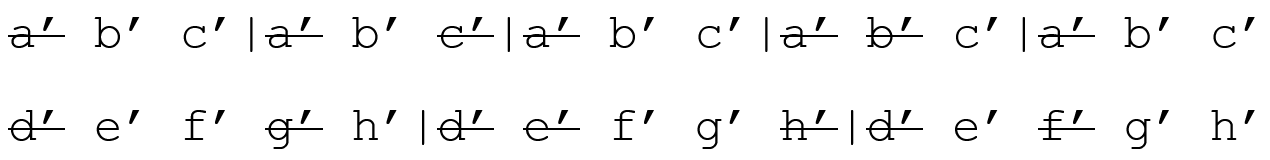
\includegraphics[width=\textwidth]{diagram.png}};
    \end{tikzpicture}
    \caption{Legendre symbol of residues from 0 to 14 modulo 3 and 5. Multiples of 3 or 5 are crossed out.}
\end{figure}
Let $(a', b', c') = (\qrn{0}{3}, \qrn{1}{3}, \qrn{2}{3})$, and $(d', e', f', g', h') = (\qrn{0}{5}, \cdots, \qrn{4}{5})$. In order to have $\qrB{p}{q}\qrB{p}{r}$ be constant, the product of the elements in each non-crossed-out column has to be equal, because due to the surjectivity lemma, the sequence $bk+c$ only covers all columns that contains neither $a'$ or $d'$. Then, when varying $p=bk+c$ by increasing $k$, the expression $\qrB{p}{q}\qrB{p}{r}$ becomes $b'e', c'f', b'h', a'e',$ $b'f', c'g', b'd', c'e', b'g',$ and $c'h'$. These products must all be equal, yielding $b'e'=b'f'=b'g'=b'h' \implies e'=f'=g'=h'$. Likewise, $b'=c'$.

However, these equalities cannot be true since there are $\frac{q-1}{2}$ non-zero quadratic residues and non-residues$\pmod q$, and similarly for $r$. The same would apply for any odd primes $q, r$. Thus, both $\qrB{p}{q}$ and $\qrB{p}{r}$ have to individually be constant. \qedsymbol

The product lemma and surjectivity lemma together imply that $q \mid b$ and $r \mid b$. Then, our new family of triplets currently has the conditions $a=q^{\al_1}r^{\al_2}$ for odd $\al_1, \al_2$, $4qr | b$, and $c \equiv 3 \pmod 4$, as well as equation \ref{eq3}. To distinguish more families of triplets, we use more casework. 

If $qr \equiv 1 \pmod 4 \implies q=r=1\text{ or } q=r=3 \implies (-1)^{\frac{q+r-2}{2}}=1$, then we must choose $c$ such that $\qrB{p}{q}=\qrB{p}{r} \implies \qrB{c}{q}=\qrB{c}{r}$ to satisfy equation \ref{eq3}. Note that this does produce a family of triplets. (See family 6 in section \ref{foundfamilies}.)

Otherwise if $qr \equiv -1 \pmod 4 \implies (q,r)=(1,3)\text{ or } (3,1) \implies (-1)^{\frac{q+r-2}{2}}=-1$, then we must choose $c$ such that $\qrB{p}{q}=-\qrB{p}{r} \implies \qrB{c}{q}=-\qrB{c}{r}$. This is another family of triplets. (See family 7 in section \ref{foundfamilies}.)

\subsubsection{$\gcd(b,c)=1$, $a$ is any odd number}
Let $a=\displaystyle\prod_{i=1}^{\beta} q_{i}^{\al_i}.$
We still must create the key conditions $4 \mid b, \hspace{2pt} c \equiv 3 \pmod 4$, and $\qrB{a}{p} =1$ for all primes $p = bk+c$.
Notice that if any $\al_i$ is even, then it can be ignored by simplifying the exponent similar to in equation \ref{alphaodd}. Then, without loss of generality, we assume that all $\al_i$ are odd and then simplify the exponent as in equation \ref{alphaodd}, yielding
\[\prod_{i=1}^{\beta}\qrn{q_i}{p} = 1.\]
Applying Quadratic Reciprocity for every prime $q_i$ gives
\begin{equation}\qrbg{a}{p}=\prod_{i=1}^{\beta}\qrn{q_i}{p} = \prod_{i=1}^{\beta} (-1)^{\frac{q_i-1}{2}}\qrbg{p}{q_i}=1.\end{equation}
From a similar argument using the product and surjectivity lemmas, we must have $q_i \mid b$ for all $q_i$. We also have $4\mid b$ from a key condition, so \[4 \prod_{i=1}^{\beta} q_i \mid b.\]
Then, since \[\prod_{i=1}^{\beta} (-1)^{\frac{q_i-1}{2}}\] is constant with respect to $k$, it suffices to choose values of $c$ such that
\[\prod_{i=1}^{\beta}\qrbg{c}{q_i}=\prod_{i=1}^{\beta} (-1)^{\frac{q_i-1}{2}},\] which satisfies equation 4 and thus gives us a new family of triplets. (See family 8 in section \ref{foundfamilies}.)

In this section, we found many different family of primes by considering careful casework and then generalizing cases. This took us from finding families where $a$ is an odd prime to families where $a$ is odd.
\newpage
\subsection{Found Families of Triplets}
\label{foundfamilies}
To summarize, the families of triplets found include the following.
\newline
1. $\qrn{a}{c} = 1, \hspace{2pt} c \equiv 3 \pmod 4, \hspace{2pt} c$ is prime, and $c \mid b$. \\
2. $a \equiv 1 \pmod 4$ is an odd prime, $4a \mid b$, $c \equiv 3 \pmod 4$, and $\qrn{c}{a}=1$. \\
3. $a \equiv 3 \pmod 4$ is an odd prime, $4a \mid b$, $c \equiv 3 \pmod 4$, and $\qrn{c}{a}=-1$. \\
4. $a$ is both odd and a perfect square, $4 \mid b$ and $c \equiv 3 \pmod 4$. \\
5. $a=q^{\al} \equiv 3 \pmod 4$ where $q$ is an odd prime and $\al$ is odd, $4a \mid b$, $c \equiv 3 \pmod 4$, and $\qrn{c}{a} = 1$. \\
6. $a = q^{\al_1}r^{\al_2}$, where $q,r$ are odd primes and $\al_1, \al_2$ are odd, $4qr \mid b$, $c \equiv 3 \pmod 4$, $qr \equiv 1 \pmod 4$, and $\qrB{c}{q}=\qrB{c}{r}$. \\
7. $a = q^{\al_1}r^{\al_2}$, where $q,r$ are odd primes and $\al_1, \al_2$ are odd, $4qr \mid b$, $c \equiv 3 \pmod 4$, $qr \equiv 3 \pmod 4$, and $\qrB{c}{q}=-\qrB{c}{r}$. \\
8. $a$ is a product of odd powers of primes $q_i$ where $1 \le i \le \beta$, $4 \mid b$ and $q_i \mid b$ for each $q_i$, $c \equiv 3 \pmod 4$, and $c$ is chosen such that \[\prod_{i=1}^{\beta}\qrbg{c}{q_i}=\prod_{i=1}^{\beta} (-1)^{\frac{q_i-1}{2}}.\]
Note that these are not all possible families, since the case where $a$ is even has not been explored.

These families of triplets demonstrate that the results from section \ref{proofsimpler} can be generalized, making it much simpler to generate a wide variety of triplets $(a,b,c)$ that satisfy the problem.

However, this usage of quadratic residues has its limitations. If the proof by contradiction is invalid, there may still be a triplet that can be proven to work via a different method of proof.
\newpage
\section{Conclusion}
In this essay, number theoretic concepts were introduced, including modular arithmetic and its arithmetic operations, Euler's Totient Theorem and its corollaries, then quadratic residues and its many theorems, which were then put to use in a Taiwanese Olympiad problem and then in a problem from the mathematician Fermat. Afterwards was a deep exploration of my extension to the problem. Areas for further exploration include exploring in the extension the case where $a$ is even, and extending the Taiwanese Olympiad problem by seeking a generalization of the numbers used. 

However, I believe the purpose of this essay---to demonstrate the usefulness of quadratic residues---has been adequately achieved, as the Taiwanese Olympiad problem demonstrated how quadratic residues can be useful but has its limitations, while an extension to Fermat's problem involving families of primes has been explored in depth.
\newpage

\section{References}
[1] Silverman, Joseph. "A Friendly Introduction to Number Theory." \textit{A \\ Friendly Introduction to Number Theory}, 2012,  https://www.math.brown.edu/\\ johsilve/frint.html. Retrieved August 7, 2022.

[2] Rusczyk, Richard. “Modular Arithmetic/Introduction.” \\ \textit{Art of Problem Solving}, 2021, https://artofproblemsolving.com/wiki/index.php/\\ Modular\_arithmetic/Introduction. Retrieved August 7, 2022.

[3] “Graphing Calculator.” \textit{Desmos}. https://www.desmos.com/calculator. Retrieved August 7, 2022.

[4] Rusczyk, Richard. “Euler's Totient Function.” \textit{Art of Problem Solving}, 2021, \\ https://artofproblemsolving.com/wiki/index.php/Euler\%27s\_totient\_function. \\ Retrieved August 7, 2022.

[5] Weisstein, Eric W. "Fundamental Theorem of Arithmetic." \textit{MathWorld}, 2005, https://mathworld.wolfram.com/FundamentalTheoremofArithmetic.html. Retrieved August 7, 2022.

[6] Chorge, Shashank and Vargas, Juan "Proof of Euler's $\p$ (Phi) Function Formula," \textit{Rose-Hulman
Undergraduate Mathematics Journal: Vol. 14 : Iss. 2, Article 6}, 2013, https://scholar.rose-hulman.edu/rhumj/vol14/iss2/6/.

[7] Rusczyk, Richard. “Euler's Totient Theorem.” \textit{Art of Problem Solving}, 2021, https://artofproblemsolving.com/wiki/index.php/Euler\%27s\_Totient\_Theorem. Retrieved August 7, 2022,

[8] "Primitive Roots." \textit{Brilliant.org},  https://brilliant.org/wiki/primitive-roots/. Retrieved August 7, 2022.

[9] "Legendre Symbol." \textit{Brilliant.org}, https://brilliant.org/wiki/legendre-symbol/. Retrieved August 7, 2022.

[10] “Number of Quadratic Residues of Prime.” \textit{ProofWiki}, 2021,\\ https://proofwiki.org/wiki/Number\_of\_Quadratic\_Residues\_of\_Prime. \\ Retrieved August 7, 2022.

[11] “Euler's Criterion.” \textit{ProofWiki}, 2019, https://proofwiki.org/wiki/\\ Euler\%27s\_Criterion. Retrieved August 7, 2022.

[12] "Law of Quadratic Reciprocity." \textit{Brilliant.org}, https://brilliant.org/wiki/\\ law-of-quadratic-reciprocity/. Retrieved August 7, 2022.

[13] Andreescu, Titu, and Gabriel Dospinescu. \textit{Problems from the Book}. XYZ Press, 2010.

[14] Weisstein, Eric W. "Dirichlet's Theorem." \textit{MathWorld}, 2004, \\ https://mathworld.wolfram.com/DirichletsTheorem.html. Retrieved August 7, 2022.
\newpage
\section{Appendix A: Euler's Totient Theorem}
Suppose we have $a^b \pmod m$, $a, b \in \Z, m \in \Z^+$ and wish to simplify the exponent when $m$ is not a prime, so Fermat's Little Theorem does not apply. This can be done through Euler's Totient Theorem\footnote{[7] Rusczyk.}, but Euler's Totient Function must first be defined.

Define Euler's Totient Function\footnote{[4] Rusczyk.} $\p(n)$ as the number of positive integers between 1 and $n$ inclusive that are coprime to $n$. For example, the 4 positive integers less than or equal to 10 that are coprime to $10$ are 1, 3, 7, and 9, so $\p(10)=4$.

Euler's Totient Theorem states that for $a, m \in \Z^+$ such that $\gcd(a,m) = 1$, \[a^{\p(m)} \equiv 1 \pmod m.\]

\begin{comment}
\subsection{Direct Evaluation}
We wish to find a formula for $\p(n)$. Suppose that \[n=\prod_{i=1}^k p_i^{\al_i} = p_1^{\al_1}p_2^{\al_2}p_3^{\al_3}\cdots p_{k}^{\al_k},\]
where each $p_i$ for $1 \le i \le k$ are the prime factors of $n$ and thus $\al_i \ge 1$ for $1 \le i \le k$. Note that $n$ can always be expressed as such due to the Fundamental Theorem of Arithmetic\footnote{The Fundamental Theorem of Arithmetic states that every positive integer greater than 1 can be expressed as a product of 1 or more prime factors. See reference [5].}. Then, we wish to prove Euler's product formula which states that \[\p(n) = \prod_{i=1}^k (p_i-1)p_i^{\al_i-1} = (p_1-1)p_1^{\al_1 - 1} (p_2-1)p_2^{\al_2-1} \cdots (p_k - 1)p_k^{\al_k-1}.\] This will be proven by using two lemmas.\footnote{This proof follows the structure of Chorge's and Vargas's paper. See reference [6].}
\paragraph{Lemma 1}: If $p$ is a prime factor of $n$, then $\p(pn) = p\p(n)$.
\paragraph{Proof}: Consider the set of all positive integers from $1$ to $n$. Then, consider the set of numbers from $nx+1$ to $nx+n=n(x+1)$. In particular, let $m=nx+k$ for $1\le k \le n$. We use the Extended Euclidean Algorithm which states that for $a,b \in \Z^+$, $\gcd(a,b)=\gcd(a, b \pmod a)$. This gives $\gcd(n, nx+k) = \gcd(n, k)$. Notice for a specific value of $x$, there are an equal number of integers in $\{1,2,\cdots,n\}$ coprime to $n$ as integers in $\{nx+1, nx+2, \cdots, n(x+1)\}$ coprime to $n$. Since there are $p$ possible values of $x$, we have $\p(pn) = p\p(n)$.
\paragraph{Lemma 2}: If $p$ is not a prime factor of $n$, then $\p(pn)=(p-1)\p(n)$.
\paragraph{Proof}: We first take the set of integers from $1$ to $pn$ that are coprime to $n$. From similar work in Lemma 1, this is equal to $p\p(n)$. Let the integers $\{n_1, n_2, \cdots, n_{\p(n)}\}$ be the set of integers from $1$ to $n$ that are coprime to $n$. Then, the integers $\{pn_1, pn_2, \cdots, pn_{\p(n)}\}$ is a subset of the set of integers coprime to $n$ from $\{1, 2, \cdots, pn\}$. Then, to count the number of elements coprime to $pn$ from $\{1, 2, \cdots, pn\}$, we take all elements coprime to $n$ and then remove the remaining elements divisible by $p$. This is the difference of the sizes of the two sets mentioned above, which is $p\p(n)-\p(n) = (p-1)\p(n)$.

These two lemmas can be used in conjunction. Let \[n=\prod_{i=1}^k p_i^{\al_{i}},\]
where $\al_i \ge 1$. Then, Lemma 1 can be applied  $\al_i-1$ times on prime $p_i$ and Lemma 2 can be applied once to get \[\p(n)=(p_1-1)p_1^{\al_1-1} \p\left(\prod_{i=2}^k p_i^{\al_i}\right).\] Noting that $\p(1)=1$, the process above can be applied recursively to give
\[\p(n) = \prod_{i=1}^k (p_i-1)p_i^{\al_i-1}.\]
\end{comment}

Notice that as a consequence of Euler's Totient Theorem, when trying to simplify $a^b \pmod m$, we have \[a^b \pmod m \equiv a^{b + k\p(m)} \pmod m\] for any $k \in \Z$. Then, the minimum exponent that $a^b$ can be simplified to is the remainder when $b$ is divided by $\p(m)$. Notice how unlike the 4 operations in the previous section, simplifying the exponent must occur modulo $\p(m)$ instead of modulo $m$. For example, \[17^{17} \pmod{10} \equiv 7^{17 \bmod {\p(10)}} \equiv 7^{17 \bmod 4} \equiv 7^1 \equiv 7 \pmod{10}.\]

\begin{comment}
We will now prove this theorem to be used in this essay.

Consider the set of all residues modulo $m$ that are coprime to $m$. This can be expressed as $A = \{n_{1}, n_{2}, \cdots, n_{\p (m)}\}.$ For example, when $m=14$, the set would be $A = \{1, 3, 5, 9, 11, 13\}$. Then, let $a$ be an integer coprime to $m$.
\paragraph{Key Lemma}: The set of the residues of $B = \{an_{1}, an_2, \cdots, an_{\p(m)}\}$ is congruent to the set $A$ defined as all residues modulo $m$ that are coprime to $m$. In other words, every element of $B$ is found in $A$ and vice versa. For example, let $a = 3$. Then, it would be equivalent to proving that $B=\{1\cdot 3, 3 \cdot 3, 5 \cdot 3, 9 \cdot 3, 11 \cdot 3, 13 \cdot 3\}$ is congruent to $A$ when its residues are taken.
\paragraph{Proof}: Notice that each of the elements of both sets are coprime to $m$. Thus, $B \subseteq A$, meaning that all elements of $B$ must be contained in $A$. We will prove that if we have $an_x \equiv an_y \pmod m$, then $x = y$. This will prove uniqueness. Note that $an_x \equiv an_y \iff m \mid a(n_x - n_y).$ Since $m$ and $a$ share no common factors, we must have $m \mid n_x - n_y \iff x = y.$ Since all elements in $B$ are unique, meaning that $A$ and $B$ are the same number of unique elements. Since $B$ is fully contained in $A$, all $\p(m)$ unique elements of $B$ are in $A$, meaning that the two sets are the same.

Since the sets both have the same residues when each element is taken modulo $m$, the product of all of the elements of the two sets are the same. Then, \[\prod_{i=1}^{\p (m)} n_i \equiv \prod_{i=1}^{\p (m)} (an_i) \equiv a^{\p (m)} \prod_{i=1}^{\p (m)} n_i \iff \prod_{i=1}^{\p (m)} n_i (a^{\p(m)}-1) \equiv 0 \pmod m.\]
Since all $n_i$, $1 \le i \le \p(m)$ are coprime to $m$, we must have \[\prod_{i=1}^{\p (m)} n_i \neq 0 \pmod m.\]
Then, we must have \[a^{\p(m)} \equiv 1 \pmod m,\]
which proves Euler's Totient Theorem.
\end{comment}
\section{Appendix B: Modular inverses}
Traditional division does not exist in modular arithmetic because rational numbers are not defined. However, there are modular inverses. Suppose we have a residue $a \pmod m$. We define the modular inverse $a^{-1}$, if it exists, to be the residue modulo $m$ such that $a \cdot a^{-1} \equiv 1 \pmod m$. Notice that due to Euler's Totient Theorem, $a^{\p(m)} \equiv 1 \pmod m$ if $\gcd(a, m) = 1$. Then, $a^{-1} \equiv a^{\p(m)-1} \pmod m$. Thus, when $\gcd(a,m)=1$, $a^{-1}$ always exists.

It can be proven that there is at most one modular inverse for each element, and that $a^{-1}$ exists modulo $m$ if and only if $\gcd(a,m) = 1$. Here is the proof.

Suppose $\gcd(a,m)=k$, where $a, m, k \in \Z$ for some $k>1$. Since $k \mid m$, let $m = kx, \hspace{2pt} x \in \Z$. Then, we wish to find $a \cdot a^{-1} \equiv 1 \pmod m \iff m \mid (a \cdot a^{-1} - 1) \iff kx \mid (a \cdot a^{-1}-1)$, which must satisfy $k \mid (a \cdot a^{-1} - 1) \iff a \cdot a^{-1} \equiv 1 \pmod k$ because $k \mid m$. However, $ax \equiv 0 \pmod k$ for all $x \in \Z$, and so $a^{-1}$ does not exist when $\gcd(a,m) > 1$.

Uniqueness of a modular inverse can be proven by considering two modular inverses $a^{-1} \pmod m$, which we will let be $x, y \pmod m$. Then, we have $ax \equiv ay \equiv 1 \pmod m \implies ax-ay \equiv 0 \pmod m \implies a(x-y) \equiv 0 \pmod m$. Since $\gcd(a, m) = 1$, we must have $x-y \equiv 0 \pmod m \implies x \equiv y \pmod m$, meaning that there can only be at most one modular inverse. \qedsymbol
\newpage
\section{Appendix C: Proof that minimum exponent must divide the exponent}
Define $x$ to be the minimum exponent satisfying $a^x \equiv 1 \pmod b$, $a, x, b \in \Z$. Suppose $y$ satisfies $a^y \equiv 1 \pmod b$.

If $y=kx$, then $a^y \equiv a^{kx} \equiv (a^x)^k \equiv 1 \pmod b$. Now suppose that there is some integer $y=kx+c$ such that $1 \le c < x$ that satisfies $a^y \equiv 1 \pmod b$. Then, $a^y \equiv a^{kx+c} \equiv a^{kx} \cdot a^{c} \equiv a^c \equiv 1 \pmod b$, implying that $c$ is the minimum since $c<x$. However, we already assumed that $x$ is the minimum, and thus we have a contradiction. Then, we must have $c=0 \implies y = kx \implies x \mid y$. \qedsymbol
\newpage
\section{Appendix D: Proof that the primes in an arithmetic sequence has infinitely many primes for each non-zero residue}
We wish to prove that the primes of the form $p=bk+c$, when taken modulo an odd prime $a$ where $\gcd(a,b)=1$, covers all non-zero residues modulo $a$ infinitely many times.

I wish to apply Dirichlet's Theorem on Arithmetic Progressions\footnote{[14] Weisstein.}, which states that for $a, d \in \Z$ such that $\gcd(a,d) = 1$, there are infinitely many primes of the form $a \pmod d$, or in other words, there are infinitely many primes in the arithmetic sequence $a+kd, k \in \Z$. To do so, I must first find the arithmetic sequence for each of the residues $x$ modulo $a$.

We have $k \equiv (x-c)b^{-1} \pmod a$, meaning that $k = (x-c)b^{-1} + ay$ for $y \in \Z$. Plugging this back into $bk+c$ yields \[bk+c = b((x-c)b^{-1}+ay)+c = bb^{-1}(x-c) + aby+c \equiv x \pmod a,\] where $y$ varies and the other variables are constant. Then, for each residue $x$, we define an arithmetic progression with the common difference $ab$, and the first term $bb^{-1}(x-c)+c$. This arithmetic sequence has infinitely many primes if \\ $\gcd(ab, bb^{-1}(x-c)+c) = 1$. Since $a, b$ are coprime, the condition above is equivalent to the two conditions $\gcd(a, bb^{-1}(x-c)+c)=1$ and \\$\gcd(b, bb^{-1}(x-c)+c)=1$. Since $bb^{-1}(x-c)+c \equiv (x-c)+c \equiv x \pmod a$, this condition holds true if $x \neq 0 \pmod a$. Due to the Euclidean Algorithm, $\gcd(b, bb^{-1}(x-c)+c) = \gcd(b, c)=1$. Thus, primes of the form $bk+c$ will cover all non-zero residues modulo $a$, proving the lemma. \qedsymbol
\end{document}
